\documentclass{article}
\usepackage[english]{babel}
\usepackage{fullpage}
\usepackage{graphicx}
\begin{document}
\begin{center}
\large \textbf{CSE 564: Project Progress Report}\\
\normalsize {Jeanette Daum (jdaum), Chandrakana Nandi (cnandi) }
\end{center}
\section{Initial plan}
The goal of our project is to verify security and correctness properties for home automation systems. In our proposal, we already explained why this is an important step for including smart systems into our everyday lives. The violation of security in smart home systems could have severe consequences for its inhabitants. 

Our plan included building our own home automation platform after finding that most existing platforms are closed-source. We focus on the devices in a smart home, namely: controllers, sensors, and dumb devices. For example, a sensor would be a thermometer and a dumb device would be a room heater. The controller of the room heater would be a thermostat (note that the thermometer is usually a part of the thermostat and this is not a problem for our model) which would turn the room heater on/off depending on the value measured by the thermometer. For our project, we are concerned with security at the device level and not with the security of the communication protocols or the underlying operating system. 

We have defined three types of security and correctness policies. According to our original timeline, algorithms for statically verifying these policies were supposed to be designed before the checkpoint.

Overall, by the end of the quarter, we had planned to have a design and implemention of an abstract architecture for modelling smart systems, specify certain types of security and correctness policies for them and verify them. 

\section{Current state}
\textbf{Architecture:} Currently, we have implemented a prototype of the proposed architecture, and three case studies, and have a simulation working. We implemented the sensors to be broadcasting their values using an observer pattern where the controllers are the observers and the dependency sensors are the subjects. This is a variant of the traditional observer pattern because a controller can have multiple subjects. The sensors are made to generate random outputs in appropriate ranges and this is used to trigger the controllers to send commands to the dumb devices.  At the moment, the simulation updates the sensor values only once and the dumb devices upon receiving a command from a controller display a message indicating its ID and the action it executed. Figure~\ref{fig:classdia} shows the class diagram for the architecture. 

We would like to mention that we started implementing everything from scratch and so far, we have 1125 lines of code. \\

\begin{figure}[h]
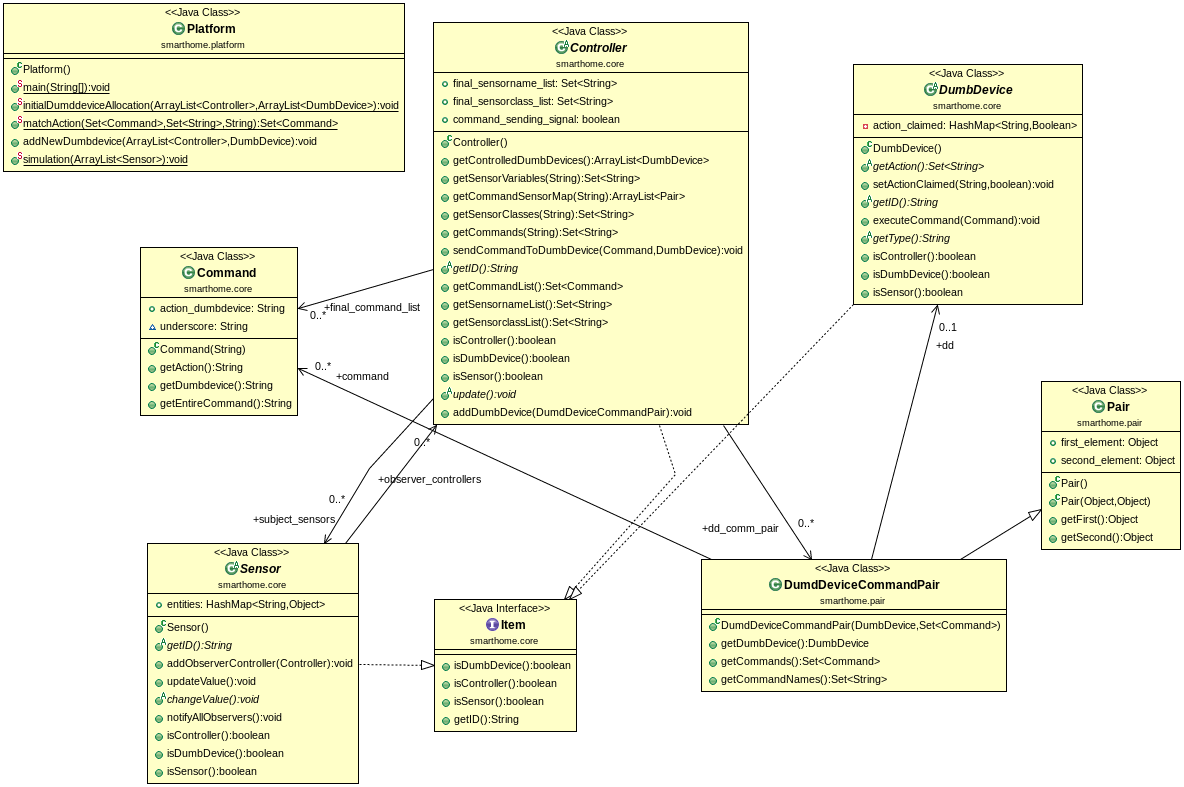
\includegraphics[scale=0.35, trim = 0 0 0 0]{classdiagram.png}
\caption{Class diagram of the home automation system}
\label{fig:classdia}
\end{figure}

\noindent \textbf{Security and correctness policies:} We have formalized three types of policies: \textit{Dependency policies}, \textit{Control policies} and \textit{New Item policy}. 

The \textit{Dependency policies} state the conditions (sensor values) under which a controller can send a command to a dumb device. They are written in separate policy files in xml format
and are currently verified by dynamic checks. 

The \textit{Control policies} state that a controller should only send commands to those dumb devices that they are supposed to control. Every controller has a list of dumb devices they can control which is stored in a special data structure we implemented for this: \texttt{DumbDeviceCommandPair}. At the moment, this policy is also checked dynamically.

The \textit{New Item policy} states that as long as all the existing controllers in the house are verified, when a new device is added, the only thing to be done to ensure that the entire home is verified is to verify the new device. Further, this verification is only needed when the new device is a controller. 
The algorithm for verifying the new item policy is:\\
\noindent Let \texttt{verify\_dependency\_policy} and \texttt{verify\_control\_policy} be methods for verifying the dependency and control policies respectively.
Then the policy states that: \\

\noindent \texttt{if (new\_device.type = sensor) \{ \\ \hspace*{1cm} no\_action; \} \\
if (new\_device.type = dumb-device) \{ \\ \hspace*{1cm} no\_action; \} \\
if (new\_device.type = controller) \{ \\ \hspace*{1cm} verify\_dependency\_policy (new\_device); \\ \hspace*{1.0cm} verify\_control\_policy (new\_device); \}}\\ 

\section{Future plans and revision of milestones}
We had planned to have the algorithms for verifying all three policies by the checkpoint but we are still trying to do so for the dependency and control policies. While the dynamic checking has been implemented already, we are looking for the best way to approach the static verification problem. Thus, our plan for the next few weeks is to focus on the verification part of the project. We did not expected it to be as complex as it seems right now. We plan to look at existing techniques such as using the Java Path Finder, or generating the Abstract Syntax Tree of the code and analysing it, or doing a data flow analysis. The reason why this part of the project is hard is because almost none of the existing program analysis tools can be used off the shelf. They need to be manually configured to handle specific problems in a project. 

We might need to revise our initial milestones because even verifying one of the three policies will be very time consuming.  Thus, our new goal is to try to implement the verification tools for at least one of the above three policies and show them working for at least one case study. After that, if we still have time, we will show it working for more case studies and also implement the tools for verifying the other two policies.

\end{document}